\documentclass[compress,red]{beamer}
\usepackage{etex}
\mode<presentation>
\setbeamertemplate{navigation symbols}{}
\usetheme{Warsaw}
%\setbeameroption{show notes}
\setbeameroption{hide notes}

%\hypersetup{pdfpagemode=FullScreen} % makes your presentation go automatically to full screen
\useoutertheme[subsection=false]{smoothbars}

% include packages
\usepackage{subfigure}
\usepackage{multicol}
\usepackage{amsmath}
\usepackage{epsfig}
\usepackage{graphicx}
\usepackage[all,knot]{xy}
\xyoption{arc}
\usepackage{url}
\usepackage{multimedia}
\usepackage{hyperref}
\usepackage{helvet}
\usepackage[polish,english]{babel}
\usepackage[utf8]{inputenc}
\usepackage{multirow}
\usepackage{verbatim}
%\usepackage{geometry}
%\geometry{verbose,letterpaper}
%\usepackage{movie15}
%\usepackage{hyperref}
\usepackage{pgfpages}


%\logo{}
\titlegraphic{\scalebox{4}{
    
\includegraphics[height=0.5cm]{../pictures/ohwr_logo.eps}
  }
}


\title % (optional, use only with long paper titles)
{F*WATCH, making a watch differently!}


\author % (optional, use only with lots of authors)
{Matthieu Cattin, Federico Vaga}
% - Give the names in the same order as the appear in the paper.
% - Use the \inst{?} command only if the authors have different
%   affiliation.

%\institute%[Universities of Somewhere and Elsewhere] % (optional, but mostly needed)
%{
  %\inst{1}%
  %BE-CO Hardware and Timing section\\
  %CERN, Geneva, Switzerland
 %\and
 %\inst{2}%
 %Department of Theoretical Philosophy\\
 %University of Elsewhere
% }
% - Use the \inst command only if there are several affiliations.
% - Keep it simple, no one is interested in your street address.

\date %(optional, should be abbreviation of conference name)
{FOSDEM, Brussels, 31 January 2015}
% - Either use conference name or its abbreviation.
% - Not really informative to the audience, more for people (including
%   yourself) who are reading the slides online

%\subject{Theoretical Computer Science}
% This is only inserted into the PDF information catalog. Can be left
% out.


% If you have a file called "university-logo-filename.xxx", where xxx
% is a graphic format that can be processed by latex or pdflatex,
% resp., then you can add a logo as follows:

%\pgfdeclareimage[height=1cm]{ohr-logo}{ohr_logo.jpg}
%\logo{\pgfuseimage{ohr-logo}}


% Delete this, if you do not want the table of contents to pop up at
% the beginning of each subsection:
\AtBeginSection[]
{
  \begin{frame}<beamer>{Outline}
    \tableofcontents[currentsection]
  \end{frame}
}


% If you wish to uncover everything in a step-wise fashion, uncomment
% the following command:

%\beamerdefaultoverlayspecification{<+->}


\begin{document}

\begin{frame}
  \titlepage
  \note[item]{Introduce speakers.}
  \note[item]{We're going to talk about a after-work project we made last summer with a few other colleagues from CERN.}
\end{frame}

\begin{frame}{Outline}
  \tableofcontents
  % You might wish to add the option [pausesections]
  \note[item]{First blabla}
  \note[item]{Then ...}
  \note[item]{Then ...}
  \note[item]{Also ...}
  \note[item]{Finally, ...}
\end{frame}


% Structuring a talk is a difficult task and the following structure
% may not be suitable. Here are some rules that apply for this
% solution:

% - Exactly two or three sections (other than the summary).
% - At *most* three subsections per section.
% - Talk about 30s to 2min per frame. So there should be between about
%   15 and 30 frames, all told.

% - A conference audience is likely to know very little of what you
%   are going to talk about. So *simplify*!
% - In a 20min talk, getting the main ideas across is hard
%   enough. Leave out details, even if it means being less precise than
%   you think necessary.
% - If you omit details that are vital to the proof/implementation,
%   just say so once. Everybody will be happy with that.



%#####################################################################
%############ SECTION ################################################
\section{Introduction}

\subsection*{} % dummy subsection to display dots

%------------ FRAME --------------------------------------------------
\begin{frame}{Why making another watch?}

  \begin{block}{Gift}
    \begin{itemize}
%    \item 
    \item for a retiring colleague
    \end{itemize}
  \end{block}

\end{frame}

%------------ FRAME --------------------------------------------------
\begin{frame}{What is it?}


\end{frame}


%#####################################################################
%############ SECTION ################################################
\section{The design}

\subsection*{} % dummy subsection to display dots

%------------ FRAME --------------------------------------------------
\begin{frame}{Mechanical design}

  \begin{block}{CAD tool selection}
    \begin{itemize}
    \item ...
    \end{itemize}
  \end{block}

  \begin{center}
    
\includegraphics[height=1cm]{../pictures/freecad_logo.eps}
  \end{center}

\end{frame}

%------------ FRAME --------------------------------------------------
\begin{frame}{Component selection}

  \begin{block}{Criteria}
    \begin{itemize}
    \item Low power consumption
    \item Available from main suppliers
    \item Small footprint
    \item ...
    \end{itemize}
  \end{block}

  \note[item]{}

\end{frame}

%------------ FRAME --------------------------------------------------
\begin{frame}{GPS module}

  \begin{block}{M10478-A1}
    \begin{itemize}
    \item Antenova
    \item 13 x 9.5 x 1.8mm
    \item Integrated antenna
    \end{itemize}
  \end{block}

  \begin{center}
    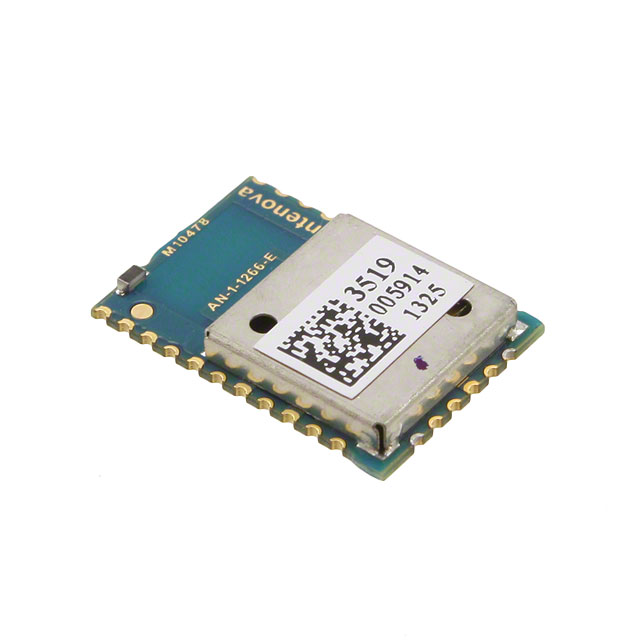
\includegraphics[height=5cm]{../pictures/M10478-A1.eps}
  \end{center}

  \note[item]{}

\end{frame}

%------------ FRAME --------------------------------------------------
\begin{frame}{Altimeter module (pressure sensor)}

  \begin{block}{MS5806-02BA}
    \begin{itemize}
    \item Measurement Specialties
    \item 6.4 x 4 x 2.8mm
    \item Water resistant
    \end{itemize}
  \end{block}

  \begin{center}
    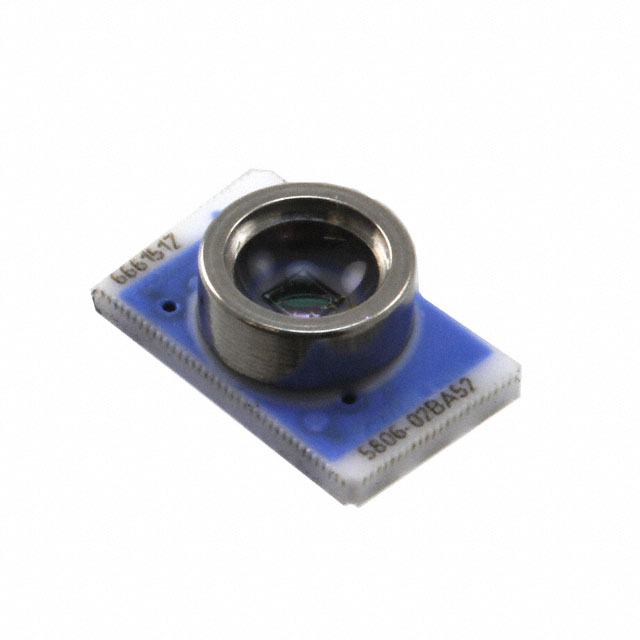
\includegraphics[height=4.5cm]{../pictures/MS5806-02BA52-51.eps}
  \end{center}

  \note[item]{}

\end{frame}

%------------ FRAME --------------------------------------------------
\begin{frame}{Display}

  \begin{block}{Memory LCD}
    \begin{itemize}
    \item Sharp
    \item 128 x 128 pixels (1.28 inches)
    \item Ultra low current
    \end{itemize}
  \end{block}


  \begin{center}
    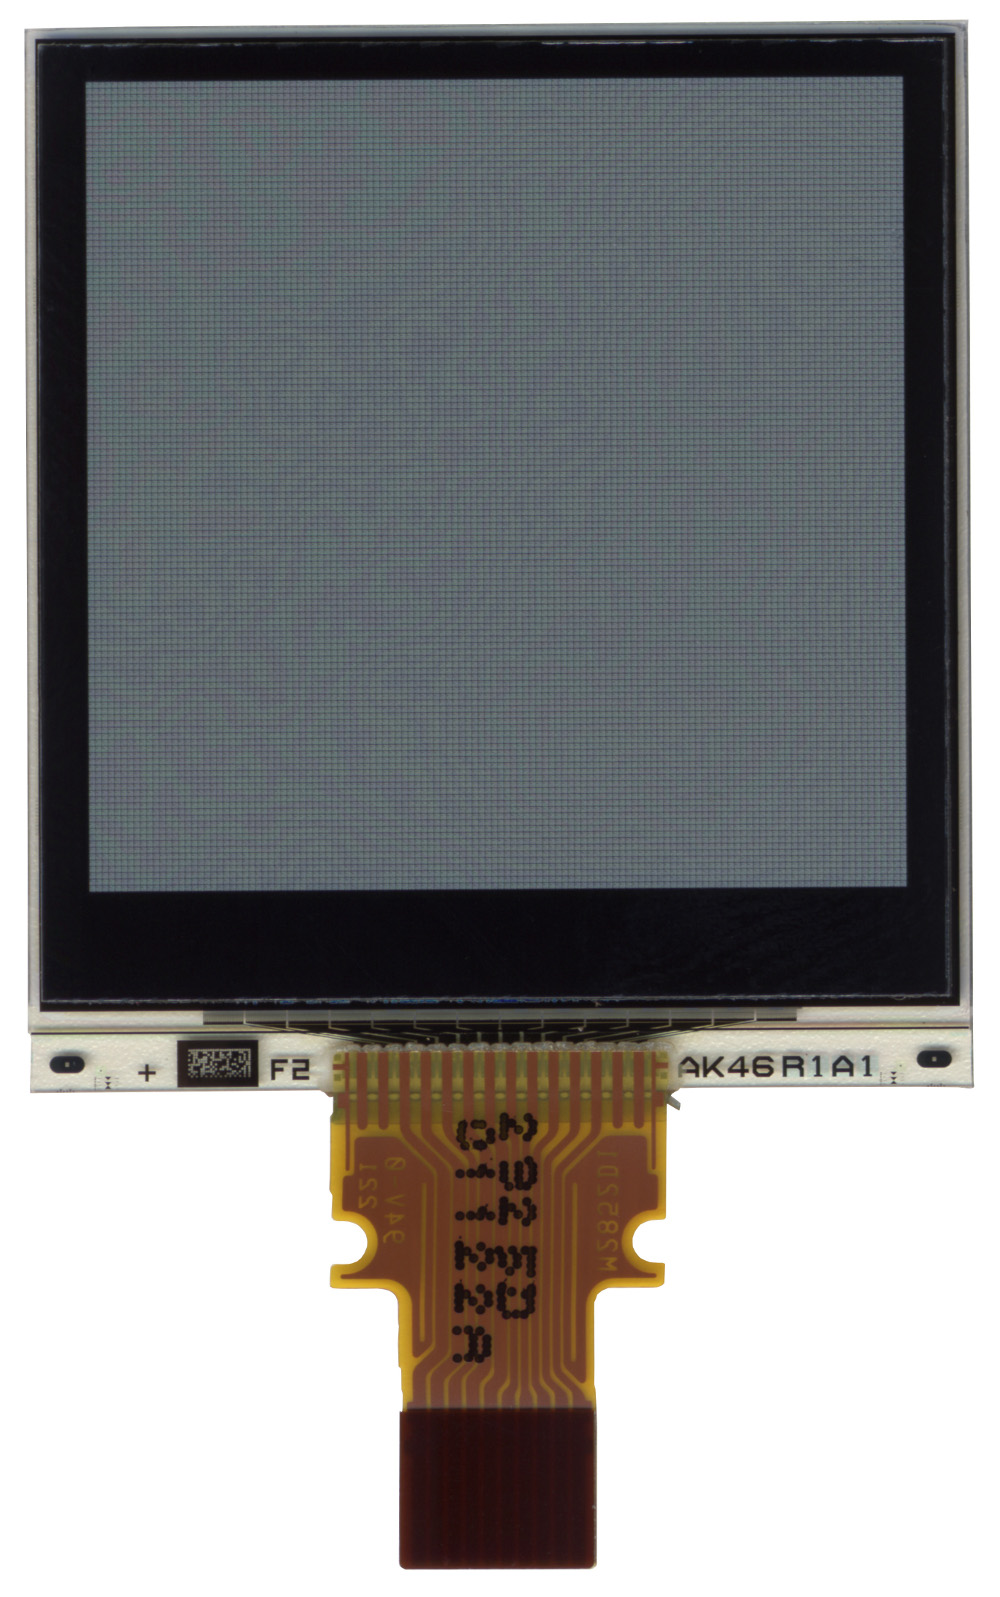
\includegraphics[height=4.5cm]{../pictures/LCD.eps}
  \end{center}

  \begin{center}

  \end{center}

  \note[item]{}

\end{frame}

%------------ FRAME --------------------------------------------------
\begin{frame}{Battery}

  \begin{block}{}
    \begin{itemize}
    \item Adafruit
    \item Li-ion 500mAh
    \item Lightweight, big capacity
    \end{itemize}
  \end{block}

  \begin{center}
    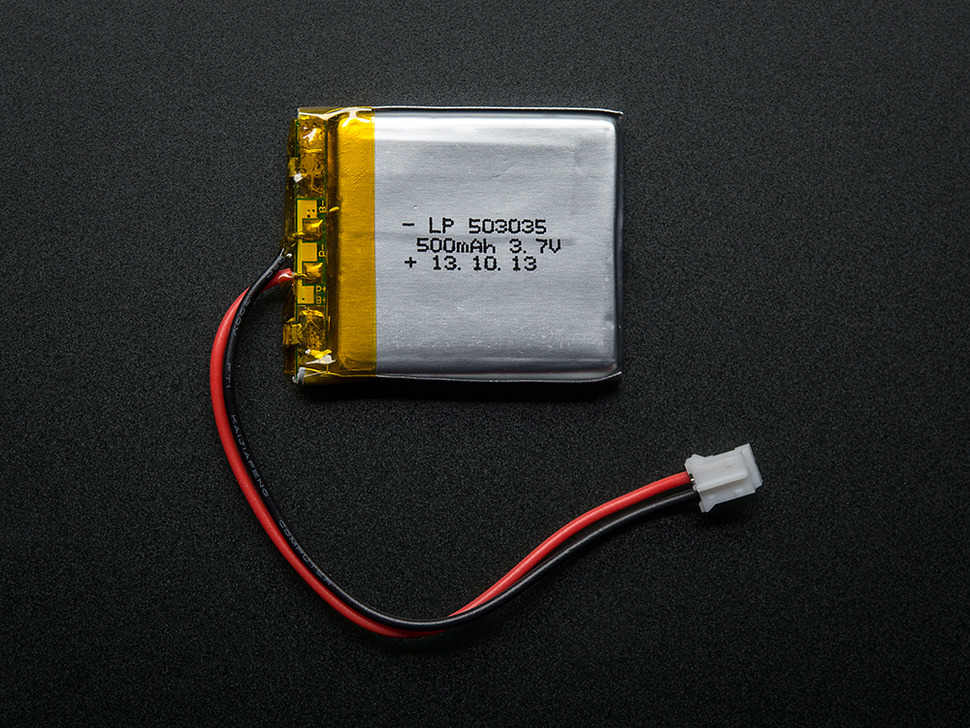
\includegraphics[height=5cm]{../pictures/battery.eps}
  \end{center}

  \begin{center}

  \end{center}

  \note[item]{}

\end{frame}

%------------ FRAME --------------------------------------------------
\begin{frame}{PCB design}

  \begin{block}{EDA tool choice}
    \begin{itemize}
    \item KiCad
    \item CERN is contributing
    \item Developer next door (help, bugfix, feedback)
    \end{itemize}
  \end{block}

  \begin{center}
    
\includegraphics[height=1cm]{../pictures/kicad_logo.eps}
  \end{center}

  \note[item]{}

\end{frame}

%------------ FRAME --------------------------------------------------
\begin{frame}{Software (firmware, host software)}

  \begin{center}
    %\includegraphics[height=7cm]{../pictures/spec_v4.eps}
  \end{center}

  \note[item]{}

\end{frame}


%#####################################################################
%############ SECTION ################################################
\section{The tools / the message}

\subsection*{} % dummy subsection to display dots

%------------ FRAME --------------------------------------------------
\begin{frame}{Mecahnical design}

  \begin{block}{Wishbone for modularity}
    \begin{itemize}
    \item Open standard
    \item Simple, uses few FPGA resources
    \item Collection of cores already available (OpenCores)
    \end{itemize}
  \end{block}

  \begin{block}{New cores developed}
    \begin{itemize}
    \item At CERN: VME64x, PCIe, DDR3
    \item By collaborators: Wishbone crossbar (GSI)
%    \item Crossbar to interconnect/arbitrate masters and slaves % developed in GSI
    \end{itemize}
  \end{block}

  \note[item]{}

\end{frame}

%------------ FRAME --------------------------------------------------
\begin{frame}{PCB design}

  \begin{center}
    %\includegraphics[height=6cm]{../pictures/spec-fmc-adc_arch_simple_color.eps}
  \end{center}

  \note[item]{}

\end{frame}

%------------ FRAME --------------------------------------------------
\begin{frame}{Software}

  \begin{center}
    %\includegraphics[height=6cm]{../pictures/spec-fmc-adc_arch_simple_color.eps}
  \end{center}

  \note[item]{}

\end{frame}


%#####################################################################
%############ SECTION ################################################
\section{Building a watch}

\subsection*{} % dummy subsection to display dots

%------------ FRAME --------------------------------------------------
\begin{frame}{I want to build this watch, what should I do?}

  \begin{block}{hdlmake: Automating HDL design flow}
    \begin{itemize}
    \item Generates Makefiles for synthesis and simulation.
    \item Project structure described in Manifest files.
    \item Solves dependencies (fetches remote ones).
    \end{itemize}
  \end{block}

  \begin{block}{wbgen2: Wishbone slave generator}
    \begin{itemize}
    \item Describes structure in a single text file.
    \item Automatically generates HDL source, C header and documentation.
    \item Generates registers, RAM, FIFO, interrupt controller.
    \end{itemize}
  \end{block}

  \begin{block}{}
    \begin{center}
      Both FOSS tools available on ohwr.org
    \end{center}
  \end{block}

  \note[item]{}

\end{frame}


%#####################################################################
%############ SECTION ################################################
\section{What's next?}

\subsection*{} % dummy subsection to display dots

%------------ FRAME --------------------------------------------------
\begin{frame}{Future work}

  \begin{block}{Consolidate our designs}
    \begin{itemize}
%    \item Consolidate gateware and drivers. Make more releases.
%    \item Consolidate documentation (manuals, FAQs, ...).
%    \item Help companies to provide support.
%    \item Cleanup and unify repositories.
    \item Consolidate documentation (starter guides, ...).
    \item Continue to tranfer knowledge to companies. 
    \end{itemize}
  \end{block}

  \begin{block}{Future platform}
    \begin{itemize}
    \item Current platform limitations
    \item Ready for a new platform
      \begin{itemize}
%      \item Just designing a carrier
      \item Re-useable mezzanines set
      \item HDL and software framework ready
      \end{itemize}
    \end{itemize}
  \end{block}

  \note[item]{}

\end{frame}


%------------ FRAME --------------------------------------------------
\begin{frame}{Conclusions}

  \begin{block}{}
    \begin{itemize}
    \item CERN's FMC kit is not only a set of hardware modules.
      \begin{itemize}
      \item Collection of HDL cores
      \item Linux device drivers, libraries and test programs
      \item Production test systems
      \item Tools and concepts %(wbgen, hdlmake, )
       \end{itemize}
%    \item Commercially available (sometimes from several sources)
    \item Using standards improves re-usability. %(VME64x, PCIe, FMC, Wishbone)
    \item Eight CERN designs are already commercialized.
    \item New users and collaborations are welcome.
    \item Four years of experience show it works!

%    \item Open Hardware has many advantages.
%      \begin{itemize}
%      \item Anyone can help in developments and make improvements.
%      \item Allows to work differently with industry. % (design work, smaller companies).
%      \item Not tied to a single company for production and support.
%      \end{itemize}
%    \item OHR site is practical for engineers and is stimulating.
%    \item OHR site contains many re-usable HDL cores.
%    \item Good FOSS tools needed to facilitate sharing.
%    \item Many designs being developed and several are already produced by industry.
    \end{itemize}
  \end{block}

  \note[item]{}

\end{frame}

%------------ FRAME --------------------------------------------------
\begin{frame}{Open products are real products\textsuperscript{\texttrademark}}

  \begin{center}
    %\includegraphics[height=6cm]{../pictures/ohr_companies.eps}
  \end{center}

  \begin{block}{}
    \begin{center}
    Want to know more? Take a tour on \textbf{ohwr.org}
    \end{center}
  \end{block}

  \note[item]{}

\end{frame}




\begin{comment}


\end{comment}


\end{document}


